\documentclass[_ArquivoPrincipal.tex]{subfiles}

\begin{document}

%==================================================================================================
\section{Conceitos Iniciais} \label{CI}
%==================================================================================================

\textcolor{red}{Comentar brevemente alguns conceitos que irão ser utilizados: notação simbólica, indicial, delta de Kronecker, permutação de Levi-Cevita, integração por partes com o Teorema da divergência}

%==================================================================================================
\subsection{Integração Temporal} \label{MEFP-IntTemp}
%==================================================================================================

Como observado no equacionamento apresentado, há o surgimento de equações diferenciais com variações temporais. No entanto a determinação de uma expressão analítica que descreva o desenvolvimento dos parâmetros ao longo do tempo é de grande dificuldade, sendo necessário o desenvolvimento de métodos numéricos que representem adequadamente aos valores que a solução possui no tempo. Nesse cenário serão apresentados na presente seção alguns métodos de integração temporal baseados em diferenças finitas, sendo eles, o método por diferenças finitas adiantado (ou explícito), atrasado (ou implícito), central (ou semi-implícito), $\alpha$-generalizado e o método de Newmark.

Para se obter a taxa de variação temporal de uma propriedade qualquer $\phi$ ($\dot{\phi}=\partial\phi/\partial t$) a partir de uma abordagem de diferenças finitas adiantadas faz-se inicialmente uma expansão em séries de Taylor da mesma:

\begin{equation}
    \phi_{n+1}=\phi_n+\left.\frac{\partial\phi}{\partial t}\right|_n\Delta t+\frac{1}{2}\left.\frac{\partial^2\phi}{\partial t^2}\right|_n\Delta t^2+\cdots\text{,}\label{eq:TaylorAd}
\end{equation}

\noindent que, truncando a série no termo de primeira ordem, obtém-se:

\begin{equation}
    \dot{\phi}_n=\left.\frac{\partial\phi}{\partial t}\right|_n\approx\frac{\phi_{n+1}-\phi_n}{\Delta t}\text{.}
\end{equation}

\noindent Logo:

\begin{equation}
    \phi_{n+1}=\phi_n+\dot{\phi}_n\Delta t\text{.}
\end{equation}

Percebe-se que para se obter o valor posterior de uma propriedade segundo essa abordagem, é necessário conhecer somente valores presentes da mesma. Portanto o resultado desse integrador é obtido explicitamente. Além disso, como a série de Taylor foi truncada no termo de primeira ordem, então a ordem de precisão alcançada por esse integrador é $\script{O}(\Delta t)$.

Já nas diferenças atrasadas procede-se de forma semelhante, no entanto utilizando um intervalo de tempo $-\Delta t$, resultando em uma expansão em série de Taylor na forma:

\begin{equation}
    \phi_{n-1}=\phi_n-\left.\frac{\partial\phi}{\partial t}\right|_n\Delta t+\frac{1}{2}\left.\frac{\partial^2\phi}{\partial t^2}\right|_n\Delta t^2-\cdots\text{,}\label{eq:TaylorAt}
\end{equation}

\noindent que, ao truncar no termo de primeira ordem, obtém-se:

\begin{equation}
    \dot{\phi}_n=\frac{\phi_n-\phi_{n-1}}{\Delta t}\therefore
    \phi_n=\phi_{n-1}+\dot{\phi}_n\Delta t\text{.}
\end{equation}

\noindent Ajustando os índices para um passo de tempo posterior, obtém-se:

\begin{equation}
    \phi_{n+1}=\phi_n+\dot{\phi}_{n+1}\Delta t\text{.}
\end{equation}

Portanto, pode-se observar que a determinação do valor posterior da propriedade depende de sua taxa de variação temporal nesse mesmo passo de tempo, sendo, assim, um procedimento implícito. E, da mesma forma que foi constatado no integrador explícito, esse possui uma ordem de precisão de $\script{O}(\Delta t)$.

Na sequência pode-se obter uma expressão que obtenha o valor da propriedade segundo uma abordagem de diferenças finitas centrais. Para isso subtrai-se \ref{eq:TaylorAt} de \ref{eq:TaylorAd}, obtendo-se:

\begin{equation}
    \phi_{n+1}-\phi_{n-1}=2\left.\frac{\partial\phi}{\partial t}\right|_n\Delta t+\frac{1}{3}\left.\frac{\partial^3\phi}{\partial t^3}\right|_n\Delta t^3+\cdots\text{,}\label{eq:TaylorCen}
\end{equation}

Como o termo de segunda ordem foi anulado, então pode-se realizar o truncamento no termo de primeira ordem sem perder a precisão obtida na segunda ordem. Assim, obtém-se que:

\begin{equation}
    \dot{\phi}_n=\left.\frac{\partial\phi}{\partial t}\right|_n\approx\frac{\phi_{n+1}-\phi_{n-1}}{2\Delta t}\text{.}
\end{equation}

\noindent Logo:

\begin{equation}
    \phi_{n+1}=\phi_{n-1}+2\dot{\phi}_n\Delta t\text{,}
\end{equation}

Também pode-se somar as equações \ref{eq:TaylorAd} e \ref{eq:TaylorAt} e fazer o truncamento no termo de primeira ordem, onde obtém-se que:

\begin{equation}
    \phi_n=\frac{\phi_{n+1}+\phi_{n-1}}{2}\text{.}
\end{equation}

Assim, trocando-se os índices $n-1\to n$ e $n\to n+1/2$ e tomando $\Delta t\to\Delta t/2$, tem-se que:

\begin{equation}
    \phi_{n+1}=\phi_n+\frac{\dot{\phi}_{n+1}+\dot{\phi}_n}{2}\Delta t\text{,}
\end{equation}

Essa solução pode ser entendida como a média entre as soluções das diferenças adiantadas com as diferenças atrasadas, possuindo uma precisão na ordem de $\script{O}(\Delta t^2)$. A Figura \ref{fig:DifFin} apresenta graficamente a interpretação das diferenças finitas adiantadas, atrasadas e centrais.

\begin{figure}[h]
    \centering
    \caption{Interpretação gráfica das diferenças finitas:}
    \begin{subfigure}{0.32\textwidth}
    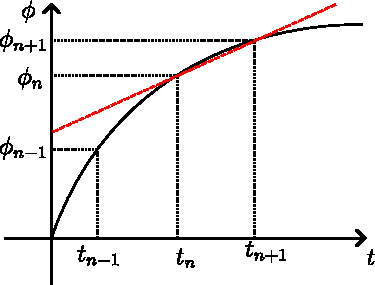
\includegraphics[width=\linewidth]{Figuras/DifAd.pdf}
    \caption{Adiantadas.}
    \end{subfigure}
    \begin{subfigure}{0.32\textwidth}
    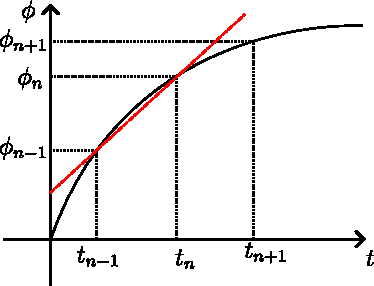
\includegraphics[width=\linewidth]{Figuras/DifAt.pdf}
    \caption{Atrasadas.}
    \end{subfigure}
    \begin{subfigure}{0.32\textwidth}
    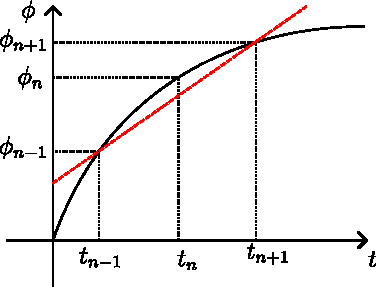
\includegraphics[width=\linewidth]{Figuras/DifCen.pdf}
    \caption{Centrais.}
    \end{subfigure}
    \\Fonte: Autoria Própria (\the\year).
    \label{fig:DifFin}
\end{figure}

Com isso, foi proposto um integrador temporal por \cite{chung1993time}, denominado de $\alpha$-generalizado. Nesse integrador, considere uma propriedade $\phi_{n+\alpha}$ de um ponto distante $\alpha\Delta t$ de $\phi_n$, sendo $0\leq\alpha\leq1$, conforme ilustrado na Figura \ref{fig:alpha-gen}.

\begin{figure}[h]
    \centering
    \caption{Esquema de uma propriedade $\phi_{n+\alpha}$.}
    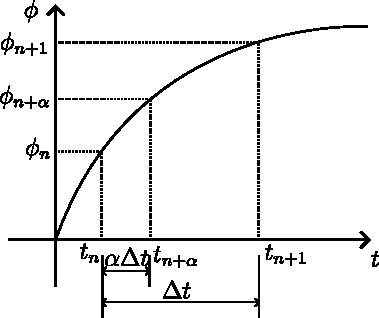
\includegraphics[width=.4\linewidth]{Figuras/alpha-gen.pdf}
    \\Fonte: Autoria Própria (\the\year).
    \label{fig:alpha-gen}
\end{figure}

Assim, pode-se realizar uma expansão em séries de Taylor:

\begin{equation}
    \phi_{n+\alpha}=\phi_n+\left.\der{\phi}{t}\right|_{n}(\alpha\Delta t)+\frac{1}{2}\left.\dder{\phi}{t}\right|_{n}(\alpha\Delta t)^2+\hdots\text{,}
    \label{eq:Taylor-alpha-gen}
\end{equation}

\noindent que, ao truncar no termo de primeira ordem pode-se obter que:

\begin{equation}
    \dot{\phi}_n=\frac{\phi_{n+\alpha}-\phi_n}{\alpha\Delta t}\text{.}
    \label{eq:der-alpha-gen}
\end{equation}

Além disso, é possível somar à Equação \ref{eq:Taylor-alpha-gen} a Equação \ref{eq:TaylorAd} e truncar no termo de primeira ordem, resultando em:

\begin{equation}
    \phi_{n+\alpha}+\phi_{n+1}=2\phi_n+(\alpha+1)\dot{\phi}_n\Delta t\text{,}
\end{equation}

\noindent que, ao substituir \ref{eq:der-alpha-gen} tem-se:

\begin{equation}
    \phi_{n+\alpha}=(1-\alpha)\phi_n+\alpha\phi_{n+1}\text{,}
\end{equation}

\noindent a qual representa uma aproximação de primeira ordem de um parâmetro $\phi_{n+\alpha}$. Em caso de uma aproximação de segunda ordem pode-se partir do truncamento a esse nível nas equações \ref{eq:TaylorAd} e \ref{eq:Taylor-alpha-gen} e seguir o procedimento análogo ao apresentado anteriormente, obtendo-se a seguinte aproximação:

\begin{equation}
    \phi_{n+\alpha}=(1-\alpha^2)\phi_n+\alpha^2\phi_{n+1}+\alpha(1-\alpha)\dot{\phi}_n\Delta t\text{.}
\end{equation}

A partir de ambas as aproximações, é possível apresentar a aproximação de Newmark, a qual aproxima valores do campo de posições ($\BB{y}$), por uma aproximação de segunda ordem, e de velocidades ($\dBB{y}$), por aproximações de primeira ordem. Para isso também descreve-se esses campos como:

\begin{subequations}
    \begin{equation}
        \BB{y}_{n+\alpha_1}=\BB{y}_n+\alpha_1\dBB{y}_n\Delta t+\frac{\alpha_1^2\ddBB{y}_{n+2\beta}\Delta t^2}{2}\text{ e}
        \label{eq:approx-pos}
    \end{equation}
    \begin{equation}
        \dBB{y}_{n+\alpha_2}=\dBB{y}_n+\alpha_2\ddBB{y}_{n+\gamma}\Delta t\text{,}
    \end{equation}
\end{subequations}

\noindent nas quais $\gamma$ e $\beta$ são parâmetros livres que podem ser calibrados em função do problema estudado e sendo a aproximação do campo de acelerações ($\ddBB{y}_{n+\gamma}$) dado por:

\begin{equation}
    \ddBB{y}_{n+\gamma}=(1-\gamma)\ddBB{y}_n+\gamma\ddBB{y}_{n+1}\text{.}
\end{equation}

Assim, realizando a simplificação do campo de velocidades tem-se:

\[
    \dBB{y}_{n+\alpha_2}=\dBB{y}_n+\alpha_2\ddBB{y}_{n+\gamma}\Delta t=\alpha_2\dBB{y}_{n+1}+(1-\alpha_2)\dBB{y}_n\text{,}
\]

\noindent que resulta em:

\begin{equation}
    \dBB{y}_{n+1}=\dBB{y}_n+\bigpar{(1-\gamma)\ddBB{y}_n+\gamma\ddBB{y}_{n+1}}\Delta t\text{.}
\end{equation}

De forma análoga tem-se, a partir da Equação \ref{eq:approx-pos} e da aproximação de segunda ordem, para o campo de posições:

\begin{equation}
    \BB{y}_{n+1}=\BB{y}+\dBB{y}_n\Delta t+\bigpar{\bigpar{\frac{1}{2}-\beta}\ddBB{y}_n+\beta\ddBB{y}_{n+1}}\Delta t^2\text{.}
\end{equation}

Verifica-se que caso $\beta=1/4$ e $\gamma=1/2$ a aproximação de Newmark recai em um caso específico igual ao das diferenças centrais.

Segundo \citeonline{fernandes2020tecnica}, o método do $\alpha$-generalizado apresenta uma boa representatividade em problemas de escoamentos incompressíveis, podendo-se introduzir uma difusão numérica à marcha no tempo. Contudo, deve-se atentar-se quanto à estabilidade do integrador ao utilizá-lo em problemas dessa natureza. Para isso, considere, portanto, uma aproximação do tipo:

\begin{subequations}
    \begin{equation}
        \dot{\phi}_{n+\alpha_m}=(1-\alpha_m)\dot{\phi}_n+\alpha_m\dot{\phi}_{n+1}\text{,}
    \end{equation}
    \begin{equation}
        \phi_{n+\alpha_f}=(1-\alpha_f)\phi_n+\alpha_f\phi_{n+1}\text{ e}
    \end{equation}
    \begin{equation}
        \phi_{n+1}=\phi_n+\Delta t\bigpar{(1-\gamma)\dot{\phi}_n+\gamma\dot{\phi}_{n+1}}\text{,}
    \end{equation}
\end{subequations}

\noindent sendo $\alpha_m$, $\alpha_f$ e $\gamma$ valores reais arbitrários. De acordo com \citeonline{chung1993time,jansen2000generalized,bazilevs2013computational}, a precisão de segunda ordem dessa aproximação pode ser atingida uma vez que:

\begin{equation}
    \gamma=\frac{1}{2}+\alpha_m-\alpha_f\text{,}
\end{equation}

\noindent assim como a estabilidade incondicional pode ser obtida uma vez que:

\begin{equation}
    \alpha_m\geq\alpha_f\geq\frac{1}{2}\text{.}
\end{equation}

Ainda é possível escrever, a partir da Equação \ref{eq:one-par-stable}, $\alpha_m$ e $\alpha_f$ em termos de um parâmetro arbitrário único  ($0\leq\rho_\infty\leq1$), que representa o raio espectral de amplificação da matriz para $\Delta t\to\infty$, o qual é utilizado para controlar as dissipações de alta-frequência.

\begin{subequations}
    \begin{equation}
        \alpha_m=\frac{1}{2}\bigpar{\frac{3-\rho_\infty}{1+\rho_\infty}}\text{ e}
    \end{equation}
    \begin{equation}
        \alpha_f=\frac{1}{1+\rho_\infty}\text{.}
    \end{equation}
    \label{eq:one-par-stable}
\end{subequations}

Para o caso de $\rho_\infty=1$ não ocorre a introdução de difusão numérica, enquanto para $\rho_\infty=0$ se tem a máxima dissipação de altas frequências \cite{fernandes2020tecnica}.

\textcolor{red}{Comentar sobre a estabilidade das diferenças finitas adiantadas, atrasadas e centrais}

%==================================================================================================
\subsection{Funções de Forma} \label{Mat-FF}
%==================================================================================================

Uma estratégia comumente utilizada para se resolver problemas onde não se conhece uma expressão para descrever o comportamento de uma função é aproximá-la por meio da combinação linear de outras funções conhecidas, denominadas como funções de forma $N_a(\BB{\xi})$, onde $a=1,\hdots,n_{en}$, $n_{en}$ é o número de nós do elemento e $\BB{\xi}\in\mathbb{R}^{n_{sd}}$ são as variáveis independentes da função avaliada, denominadas nesse contexto como coordenadas paramétricas do elemento $e$ no espaço paramétrico $\hat{\Omega}^e$. Para se entender melhor essa aproximação, considere uma propriedade $\phi$ que varia em função de $\BB{\xi}$, ou seja, $\phi=\phi(\BB{\xi})$, portanto, pode-se dizer que:

\begin{equation}
    \phi(\BB{\xi})=\sum_{a=1}^{n_{en}}{\phi_aN_a(\BB{\xi})}\text{,}
\end{equation}

\noindent sendo $\phi_a=\phi(\BB{\xi}_a)$. Algumas propriedades interessantes das funções de forma é a propriedade de interpolação, dada por $N_a(\BB{\xi}_b)=\delta_{ab}$, em que $\delta_{ab}$ é o delta de Kronecker, dado por:

\begin{equation}
    \delta_{ab}=\left\{
    \begin{array}{ll}
         1&\text{ se }a=b\\
         0&\text{ se }a\neq b 
    \end{array}
    \right.\text{,}
\end{equation}

\noindent e a partição da unidade, dada por:

\begin{equation}
    \sum_{a=1}^{n_{en}}{N_a(\BB{\xi})}=1\forall\BB{\xi}\in\hat{\Omega}^e\text{.}
\end{equation}

Em geral opta-se por funções de forma do tipo polinomiais, uma vez que se adéquam mais facilmente às mais variadas funções, além de ser uma classe de função simples de ser trabalhada. Nesse sentido destacam-se os polinômios de Lagrange, que para um polinômio de grau $p$ em caso unidimensional pode ser escrito como \cite{bazilevs2013computational}:

\begin{equation}
    l_i^p(\xi)=\prod_{j=1,j\neq i}^{p+1}{\frac{\xi-\xi_j}{\xi_i-\xi_j}}\text{, para }i=1,2,\hdots,p+1\text{.}
\end{equation}

A Figura \ref{fig:funcaoforma} apresenta graficamente a mudança de coordenada de um espaço paramétrico para um plano $x_1x_2$, de forma que $\BB{x}=\BB{x}(\xi)$.

\begin{figure}[h]
    \centering
    \caption{Mudança de espaço paramétrico para um plano $x_1x_2$.}
    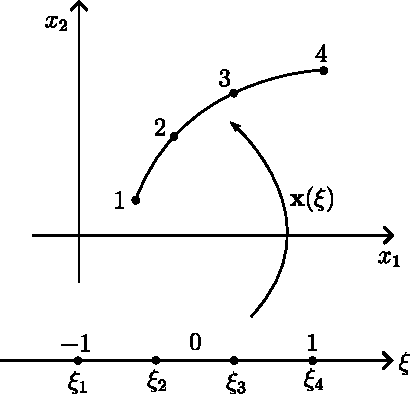
\includegraphics[width=.4\linewidth]{Figuras/funcaoforma.pdf}
    \\Fonte:Autoria Própria (\the\year).
    \label{fig:funcaoforma}
\end{figure}

\textcolor{red}{Comentar sobre funções de forma para casos multidimensionais.}

%==================================================================================================
\subsection{Integração numérica} \label{MEFP-IntNum}
%==================================================================================================

Em diversos casos pode ocorrer do surgimento de integrais cuja determinação da primitiva é inviável, ou impossível. Para isso recorre-se para métodos de aproximação numérica, que sejam capazes de estimar com boa precisão os valores das mesmas. Uma boa alternativa é a aproximação por quadratura de Gauss ou a de Hammer.

A quadratura de Gauss mais comum busca aproximar uma função $f(x)$ em um intervalo $[-1,1]$ por meio da multiplicação de $f$ em pontos estratégicos ($x_i$) com um peso associado $w_i$, ou seja:

\begin{equation}
    \int_{-1}^1{f(x)dx}\approx\sum_{i=1}^n{w_if(x_i)}\text{,}
\end{equation}

\noindent na qual $n$ é o número de pontos da quadratura.

De forma simplista, pode-se realizar uma aproximação da função $f(x)$ por meio de um polinômio $P_m(x)=\sum_{k=0}^m{a_kx^k}$, no qual $a_k$ são coeficientes constantes a cada $x^k$. Assim tem-se que:

\begin{equation}
    \int_{-1}^1{\sum_{k=0}^m{a_kx^k}dx}\approx\sum_{i=1}^n{w_i\sum_{k=0}^m{a_kx_i^k}}\text{,}
\end{equation}

\noindent o que leva a:

\begin{equation}
    \sum_{k=0}^m{a_k\frac{1-(-1)^{k+1}}{k+1}}\approx\sum_{k=0}^m{a_k\sum_{i=1}^n{w_ix_i^k}}\text{.}
\end{equation}

Assim, obtem-se o seguinte sistema de equações:

\begin{equation}
    \sum_{i=1}^n{w_ix_i^k}=\frac{1-(-1)^{k+1}}{k+1}\text{,}
\end{equation}

\noindent que, ao ser resolvida, retorna os pontos de quadratura e os pesos. A Tabela \ref{tab:QGauss} apresenta os pontos de quadratura e seus respectivos pesos para polinômios de até quarto grau.

\begin{table}[h]
    \centering
    \caption{Pontos da quadratura de Gauss e seus respectivos pesos.}
    \begin{tabular}{ccc}
    \hline
    $n$ & $x_i$ & $w_i$ \\ \hline
    2 & $\pm\frac{1}{\sqrt{3}}$ & 1 \\ \hline
    \multirow{2}{*}{3} & $0$ & $\frac{8}{9}$ \\
     & $\pm\sqrt{\frac{3}{5}}$ & $\frac{5}{9}$ \\ \hline
    \multirow{2}{*}{4} & $\pm\sqrt{\frac{3}{7}-\frac{2}{7}\sqrt{\frac{6}{5}}}$ & $\frac{18+\sqrt{30}}{36}$ \\
     & $\pm\sqrt{\frac{3}{7}+\frac{2}{7}\sqrt{\frac{6}{5}}}$ & $\frac{18-\sqrt{30}}{36}$ \\ \hline
    \end{tabular}
    \\Fonte: Autoria Própria (\the\year).
    \label{tab:QGauss}
\end{table}

De forma similar, a quadratura de Hammer mais comum busca aproximar a integral dentro de um domínio triangular, compreendido pelos pontos $(0,0)$, $(1,0)$ e $(0,1)$, como:

\begin{equation}
    \int_0^1\int_0^{1-x}{f(x,y)dydx}\approx\sum_{k=1}^n{w_kf(x_k,y_k)}\text{.}
\end{equation}

Fazendo uma aproximação por polinômio tem-se:

\begin{equation}
    \int_0^1\int_0^{1-x}{\sum_{i=0}^{n_x}{\sum_{j=0}^{n_y}{a_{ij}x^iy^j}}dydx}\approx\sum_{k=1}^n{w_k\sum_{i=0}^{n_x}{\sum_{j=0}^{n_y}{a_{ij}x_k^iy_k^j}}}\text{,}
\end{equation}

\noindent o que leva ao seguinte sistema de equações:

\begin{equation}
    \sum_{k=1}^n{w_kx_k^iy_k^j}=\frac{i!j!}{(i+j+2)!}\text{.}
\end{equation}

A Tabela \ref{tab:QHammer} apresenta os pontos da quadratura de Hammer para aproximação de 1 a 7 pontos.

\begin{table}[h]
    \centering
    \caption{Pontos da quadratura de Hammer e seus respectivos pesos para aproximação de 1 a 7 pontos.}
    \begin{tabular}{cccc}
    \hline
        $n$ & $x_k$ & $y_k$ & $w_k$ \\ \hline
        1 & 0,33333333333333 & 0,33333333333333 & 0,50000000000000 \\ \hline
        \multirow{3}{*}{3} & 0,16666666666667 & 0,16666666666667 & 0,16666666666667 \\
        & 0,16666666666667 & 0,66666666666667 & 0,16666666666667 \\
        & 0,66666666666667 & 0,16666666666667 & 0,16666666666667 \\ \hline
        \multirow{4}{*}{4} & 0,33333333333333 & 0,33333333333333 & -0,28125000000000 \\
        & 0,20000000000000 & 0,20000000000000 & 0,26041666666667 \\
        & 0,20000000000000 & 0,60000000000000 & 0,26041666666667 \\
        & 0,60000000000000 & 0,20000000000000 & 0,26041666666667 \\ \hline
        \multirow{6}{*}{6} & 0,44594849091597 & 0,44594849091597 & 0,11169079483901 \\
        & 0,44594849091597 & 0,10810301816807 & 0,11169079483901 \\
        & 0,10810301816807 & 0,44594849091597 & 0,11169079483901 \\
        & 0,09157621350977 & 0,09157621350977 & 0,05497587182766 \\
        & 0,09157621350977 & 0,81684757298046 & 0,05497587182766 \\
         & 0,81684757298046 & 0,09157621350977 & 0,05497587182766 \\ \hline
        \multirow{7}{*}{7} & 0,33333333333333 & 0,33333333333333 & 0,11250000000000 \\
        & 0,47014206410511 & 0,47014206410511 & 0,06619707639426 \\
        & 0,47014206410511 & 0,05971587178977 & 0,06619707639426 \\
        & 0,05971587178977 & 0,47014206410511 & 0,06619707639426 \\
        & 0,10128650732346 & 0,10128650732346 & 0,06296959027242 \\
        & 0,10128650732346 & 0,79742698535309 & 0,06296959027242 \\
        & 0,79742698535309 & 0,10128650732346 & 0,06296959027242 \\ \hline
    \end{tabular}
    \\Fonte: Autoria Própria (\the\year).
    \label{tab:QHammer}
\end{table}

\end{document}